\documentclass[12pt]{article}
\usepackage[utf8]{inputenc}
\usepackage[T1]{fontenc}
\usepackage{amssymb}
\usepackage{amsthm}
\usepackage{booktabs}
\usepackage{dcolumn}
\usepackage{multirow}
\usepackage{adjustbox}
\usepackage{subfig}
\usepackage{graphicx}
\usepackage{listings}
\usepackage{natbib}
\usepackage[obeyspaces,hyphens]{url}
\usepackage{lscape}
\usepackage{nicefrac}
\usepackage{xcolor}
\usepackage{amsmath}
\usepackage{txfonts}
\usepackage{empheq}
\usepackage{fancyhdr}
\usepackage{xurl}
\usepackage{ragged2e}
\usepackage{etoolbox}
\usepackage{tikz}
\usepackage[
    unicode=true,
    pdfencoding=auto,
    psdextra,
    plainpages=false,
    pdfpagelabels,
    pagebackref=false,
    hyperindex,
    breaklinks=true,
    colorlinks=true,
    citecolor=black,
    linkcolor=black,
    urlcolor=blue,
    filecolor=black,
    bookmarksopen=true
]{hyperref}
\usepackage[
    a4paper,
    left=18mm,
    right=18mm,
    top=16mm,
    bottom=18mm,
    headheight=15.8pt,
    headsep=4mm,
    footskip=8mm,
    includeheadfoot
]{geometry}

\pdfstringdefDisableCommands{%
  \def\textit#1{#1}%
  \def\emph#1{#1}%
  \def\textbf#1{#1}%
  \def\\{ }%
}

\newcommand{\be}{\begin{equation}}
\newcommand{\ee}{\end{equation}}
\def\ni{\noindent}
\newcommand{\bse}{\begin{subequations}}
\newcommand{\ese}{\end{subequations}}
\newcommand{\beq}{\begin{eqnarray}}
\newcommand{\eeq}{\end{eqnarray}}
\newcommand{\lb}[1]{\label{#1}}
\newcommand{\eg}{{\it e.g.\ }}
\newcommand{\ie}{{\it i.e.\ }}
\newcommand{\e}{{\mathrm{e}}}
\newcommand{\dd}{{\mathrm{d}}}
\newcommand{\R}{\mathbb{R}}
\newcommand{\N}{\mathbb{N}}
\newcommand{\Z}{\mathbb{Z}}
\newcommand{\Q}{\mathbb{Q}}
\newcommand{\C}{\mathbb{C}}
\newcommand{\ds}{\displaystyle}

\newtheorem{exercise}{Exercise}[section]
\newtheorem{definition}{Definition}[section]
\newtheorem{theorem}{Theorem}[section]
\newtheorem{example}{Example}[section]
\newtheorem{corollary}{Corollary}[section]
\newtheorem{proposition}{Proposition}[section]
\AtEndEnvironment{definition}{\par\nobreak\hfill\ensuremath{\lozenge}\par}

\newenvironment{demonstration}
{\par\noindent\textbf{Proof.}}
{\hfill$\square$\par}

\numberwithin{equation}{section}

\pagestyle{fancy}
\fancyhf{}
\fancyhead[R]{\small\itshape\nouppercase{\leftmark}}
\fancyfoot[L]{\scriptsize Osvaldo L. Santos-Pereira --- \href{mailto:olsp@if.ufrj.br}{olsp@if.ufrj.br}}
\fancyfoot[C]{\scriptsize \thepage}
\renewcommand{\headrulewidth}{0.4pt}
\renewcommand{\footrulewidth}{0.4pt}

\lstset{
  language=Python,
  basicstyle=\fontsize{10}{12}\selectfont\ttfamily,
  keywordstyle=\color{blue},
  commentstyle=\color{green!60!black},
  stringstyle=\color{red},
  showstringspaces=false,
  breaklines=true,
  frame=single,
  numbers=left,
  numberstyle=\tiny\color{gray},
  captionpos=b
}

\urlstyle{same}

\newcommand{\coverauthor}[4]{%
{\large\bfseries #1\par}
\vspace{0.02cm}
{\normalsize\href{mailto:#2}{#2}\par}
\vspace{0.02cm}
{\normalsize\color{blue}\url{#3}\par}
\vspace{0.02cm}
{\normalsize\itshape #4\par}
\vspace{0.8cm}
}

\long\def\coveraboutme#1{%
\vspace{0.3cm}
\begingroup
{\large\bfseries\color{black} About Me\par}
\vspace{0.18cm}
\small
\color{black!85}
\justifying
\setlength{\parindent}{18pt}
\setlength{\parskip}{3pt}
\setlength{\emergencystretch}{2em}
#1
\par
\endgroup
\vspace{0.5cm}
}

\newcommand{\sociallink}[2]{%
\noindent{\footnotesize\color{black!80} #1: \url{#2}\par}
}

\newcommand{\chaptercover}[4]{%
\begin{titlepage}
\thispagestyle{empty}
\raggedright
\setlength{\parindent}{0pt}
\vspace*{0.2cm}
{\fontsize{34}{40}\selectfont\bfseries #1\par}
\vspace{1.0cm}
{\fontsize{26}{30}\selectfont\bfseries #2\par}
\vspace{1.5cm}
\rule{\textwidth}{2.0pt}
\vspace{1.0cm}
#3
\vspace{0.3cm}
#4
\vfill
\end{titlepage}
}

\begin{document}

\chaptercover
{Binning Broad Statistical Distributions}
{Equal-Width, Quantile, and Logarithmic Methods}
{
\coverauthor
{Osvaldo L. Santos-Pereira}
{olsp@if.ufrj.br}
{https://ozsp12.github.io/}
{Physics Institute, Federal University of Rio de Janeiro (UFRJ)}
}
{
\coveraboutme{
\noindent
I hold a PhD in Physics from the Federal University of Rio de Janeiro (UFRJ), a Master's degree in Physics from the State University of Campinas (Unicamp), a Master's degree in Data Science and Analytics from the University of S\~ao Paulo (MBA USP-ESALQ), a postgraduate degree in Quantum Computing from SENAI-CIMATEC, and a Bachelor's degree in Physics from Unicamp.

\noindent
I am currently a Fellow Researcher at the Physics Institute of the Federal University of Rio de Janeiro (UFRJ), where I research Warp Drive Theory, Classical General Relativity, Cosmology, Econophysics, and Computational Physics. Other research interests include Wormhole Theory, Black Hole Theory, Quantum Gravity, Quantum Computing and Information, Mathematics, and Artificial Intelligence.

\noindent
I work in the private sector as a data science consultant and an artificial intelligence specialist. I conduct research projects across several industries, including education, health, medical, e-commerce, and large retail.

\vspace{0.3cm}
\sociallink{Curr\'iculo Lattes}{http://lattes.cnpq.br/6730251976463283}
\sociallink{ResearchGate}{https://www.researchgate.net/profile/Osvaldo-Santos-Pereira}
\sociallink{ORCID}{https://orcid.org/0000-0003-2231-517X}
\sociallink{Google Scholar}{https://scholar.google.com/citations?user=HIZp0X8AAAAJ&hl=en}
\sociallink{LinkedIn}{https://www.linkedin.com/in/ozsp12}
\sociallink{Substack}{https://substack.com/@olsp1982}
\sociallink{GitHub}{https://github.com/ozsp12}
\sociallink{YouTube}{https://www.youtube.com/@ozlsp12}
\sociallink{X (Twitter)}{https://x.com/ozsp12}
}
}

\section{Introduction}

Binning is one of the oldest and most useful operations in exploratory statistics: a continuous or finely resolved variable is replaced by a finite collection of intervals, and observations are summarized according to the intervals into which they fall. The construction is elementary, but its consequences are not. A histogram depends on the placement and width of its bins, and a representation that is harmless for a narrow, approximately symmetric distribution can become seriously misleading for a broad or heavy-tailed one. In particular, when observations span several orders of magnitude, equal-width bins allocate most of the available resolution to regions with almost no data while compressing the dense part of the sample into a small number of intervals. The resulting visual sparsity can be mistaken for absence of structure, and the rare-event tail can become dominated by sampling noise rather than by the underlying law.

These issues are central in the literature on power laws and broad statistical distributions. Newman \cite{Newman2005} gave a particularly clear account of the problem using synthetic power-law samples and empirical examples ranging from city populations and earthquake magnitudes to solar-flare intensities and personal fortunes. His comparison between an ordinary histogram, the same histogram in logarithmic coordinates, logarithmic binning, and the complementary cumulative distribution function remains a useful pedagogical demonstration of why tail analysis requires more than a routine histogram. A later methodological treatment by Clauset, Shalizi, and Newman \cite{ClausetShaliziNewman2009} emphasized an additional point: visual straightness on a log--log plot is not, by itself, statistical evidence for a power law. Heavy tails exhibit large fluctuations, the lower cutoff must be treated explicitly, and parameter estimation should be separated from visualization.

The same problem arises naturally in econophysics. Moura Jr. and Marcelo Byrro Ribeiro \cite{MouraRibeiro2009} analyzed Brazilian personal-income data from 1978 to 2005 and found that the complementary cumulative distribution for most of the population was well represented by a Gompertz form, while the upper-income tail was described by a Pareto power law. Their analysis is directly relevant to the present notes because income data combine a highly populated central region with a sparse upper tail. A binning strategy that is convenient near the modal region can therefore be inefficient precisely where the economically important extreme observations occur. More broadly, scale-free and heavy-tailed phenomena are recurrent in statistical physics and complex systems, where changes of representation can expose or conceal scaling regimes \cite{Sornette2006}.

The purpose of these lecture notes is not to advocate a single universal binning rule. Instead, the objective is to compare three practically important constructions---equal-width binning, quantile binning, and logarithmic binning---under controlled synthetic experiments. Exponential, lognormal, and Pareto samples are used because they provide three qualitatively different tail structures: a light exponential tail, a broad multiplicative distribution, and a genuine power-law tail. The comparison is complemented by cumulative and complementary cumulative representations, which separate distributional information from the arbitrary choice of histogram boundaries.

The remainder of these notes is organized as follows. Section~2 introduces the statistical problem, defines the exponential, lognormal, and Pareto distributions used throughout the numerical experiments, reviews probability density functions, cumulative distribution functions, and complementary cumulative distribution functions, and connects these objects with empirical examples. Section~3 develops the notion of binning, surveys several classical and modern bin-selection strategies, and then treats in greater detail the \texttt{pandas.qcut}, \texttt{pandas.cut}, and logarithmic-binning constructions. Section~4 presents the numerical results for the three binning methods, compares the empirical complementary cumulative distributions, and studies the mean value within each bin for the synthetic samples.



\section{Statistical distributions and the tail-resolution problem}

This section establishes the probabilistic setting of the numerical experiments. We first formulate the practical problem that motivates binning, then introduce the three distributions used throughout the notes, and subsequently place them in the general language of probability measures, densities, cumulative distributions, and survival functions. The central result is that the visual and numerical difficulty of binning is controlled not only by sample size but also by the rate at which probability mass moves into the tail. Exponential, lognormal, and Pareto samples therefore provide a useful progression from light-tailed to genuinely scale-free behavior.

\subsection{The problem and the distributions to be analyzed}

Consider a positive sample $x_1,\ldots,x_n$ whose values may extend over a broad dynamic range. If the interval from the sample minimum to the sample maximum is divided into $K$ intervals of equal width, then each interval receives the same geometric length but generally not the same probability mass. This distinction is minor for a relatively compact distribution and decisive for a heavy-tailed one. In a Pareto sample, a small number of extreme observations can enlarge the total range by orders of magnitude, making the equal-width partition extremely coarse near the lower cutoff and nearly empty over much of the remaining range.

The experiments in these notes use $N=10^6$ observations from three continuous distributions. The exponential sample has scale $50$, the lognormal sample has logarithmic mean $\ln 150$ and logarithmic standard deviation $0.55$, and the Pareto sample has lower cutoff $x_{\min}=100$ and probability-density exponent $\alpha=2.5$. These numerical scales are chosen to place the synthetic observations on readable income-like ranges; they do not assert that an empirical income distribution follows any one of the three laws over its entire support.

The motivation from income data is concrete. The Brazilian analysis of Moura Jr. and Ribeiro \cite{MouraRibeiro2009} separates the dominant body of the distribution from a much smaller Pareto upper tail. A uniform discretization of the entire income range can therefore spend many bins on intervals containing very few households while under-resolving the body of the distribution. This is precisely the situation in which quantile bins or geometrically expanding bins can be more informative than a single equal-width partition.

Newman's review provides a second motivation through Zipf's law, the rank--size form of power-law behavior \cite{Newman2005}. Zipf originally studied rank--frequency regularities in language and related social data \cite{Zipf1949}, while the same mathematical structure later became standard in the analysis of city sizes and other broad distributions. If a positive random variable has Pareto CCDF $\overline F(x)\propto x^{-(\alpha-1)}$, then the expected rank $r$ of an observation of size $x$ in a sample of size $n$ satisfies, to leading order,
\begin{equation}
 r\simeq n\,\overline F(x)\propto x^{-(\alpha-1)},
\end{equation}
and therefore
\begin{equation}
 x(r)\propto r^{-1/(\alpha-1)}.
\end{equation}
The classical Zipf case $x(r)\propto r^{-1}$ corresponds to a Pareto density exponent near $\alpha=2$. This equivalence between a distributional tail and a rank--size law is important for the present problem because both representations become sensitive to sparse extreme observations, although they organize the information differently. Newman's treatment makes this connection explicit and also shows why logarithmic binning and cumulative representations are useful when the empirical tail spans several orders of magnitude \cite{Newman2005}.

\begin{figure}[!t]
\centering
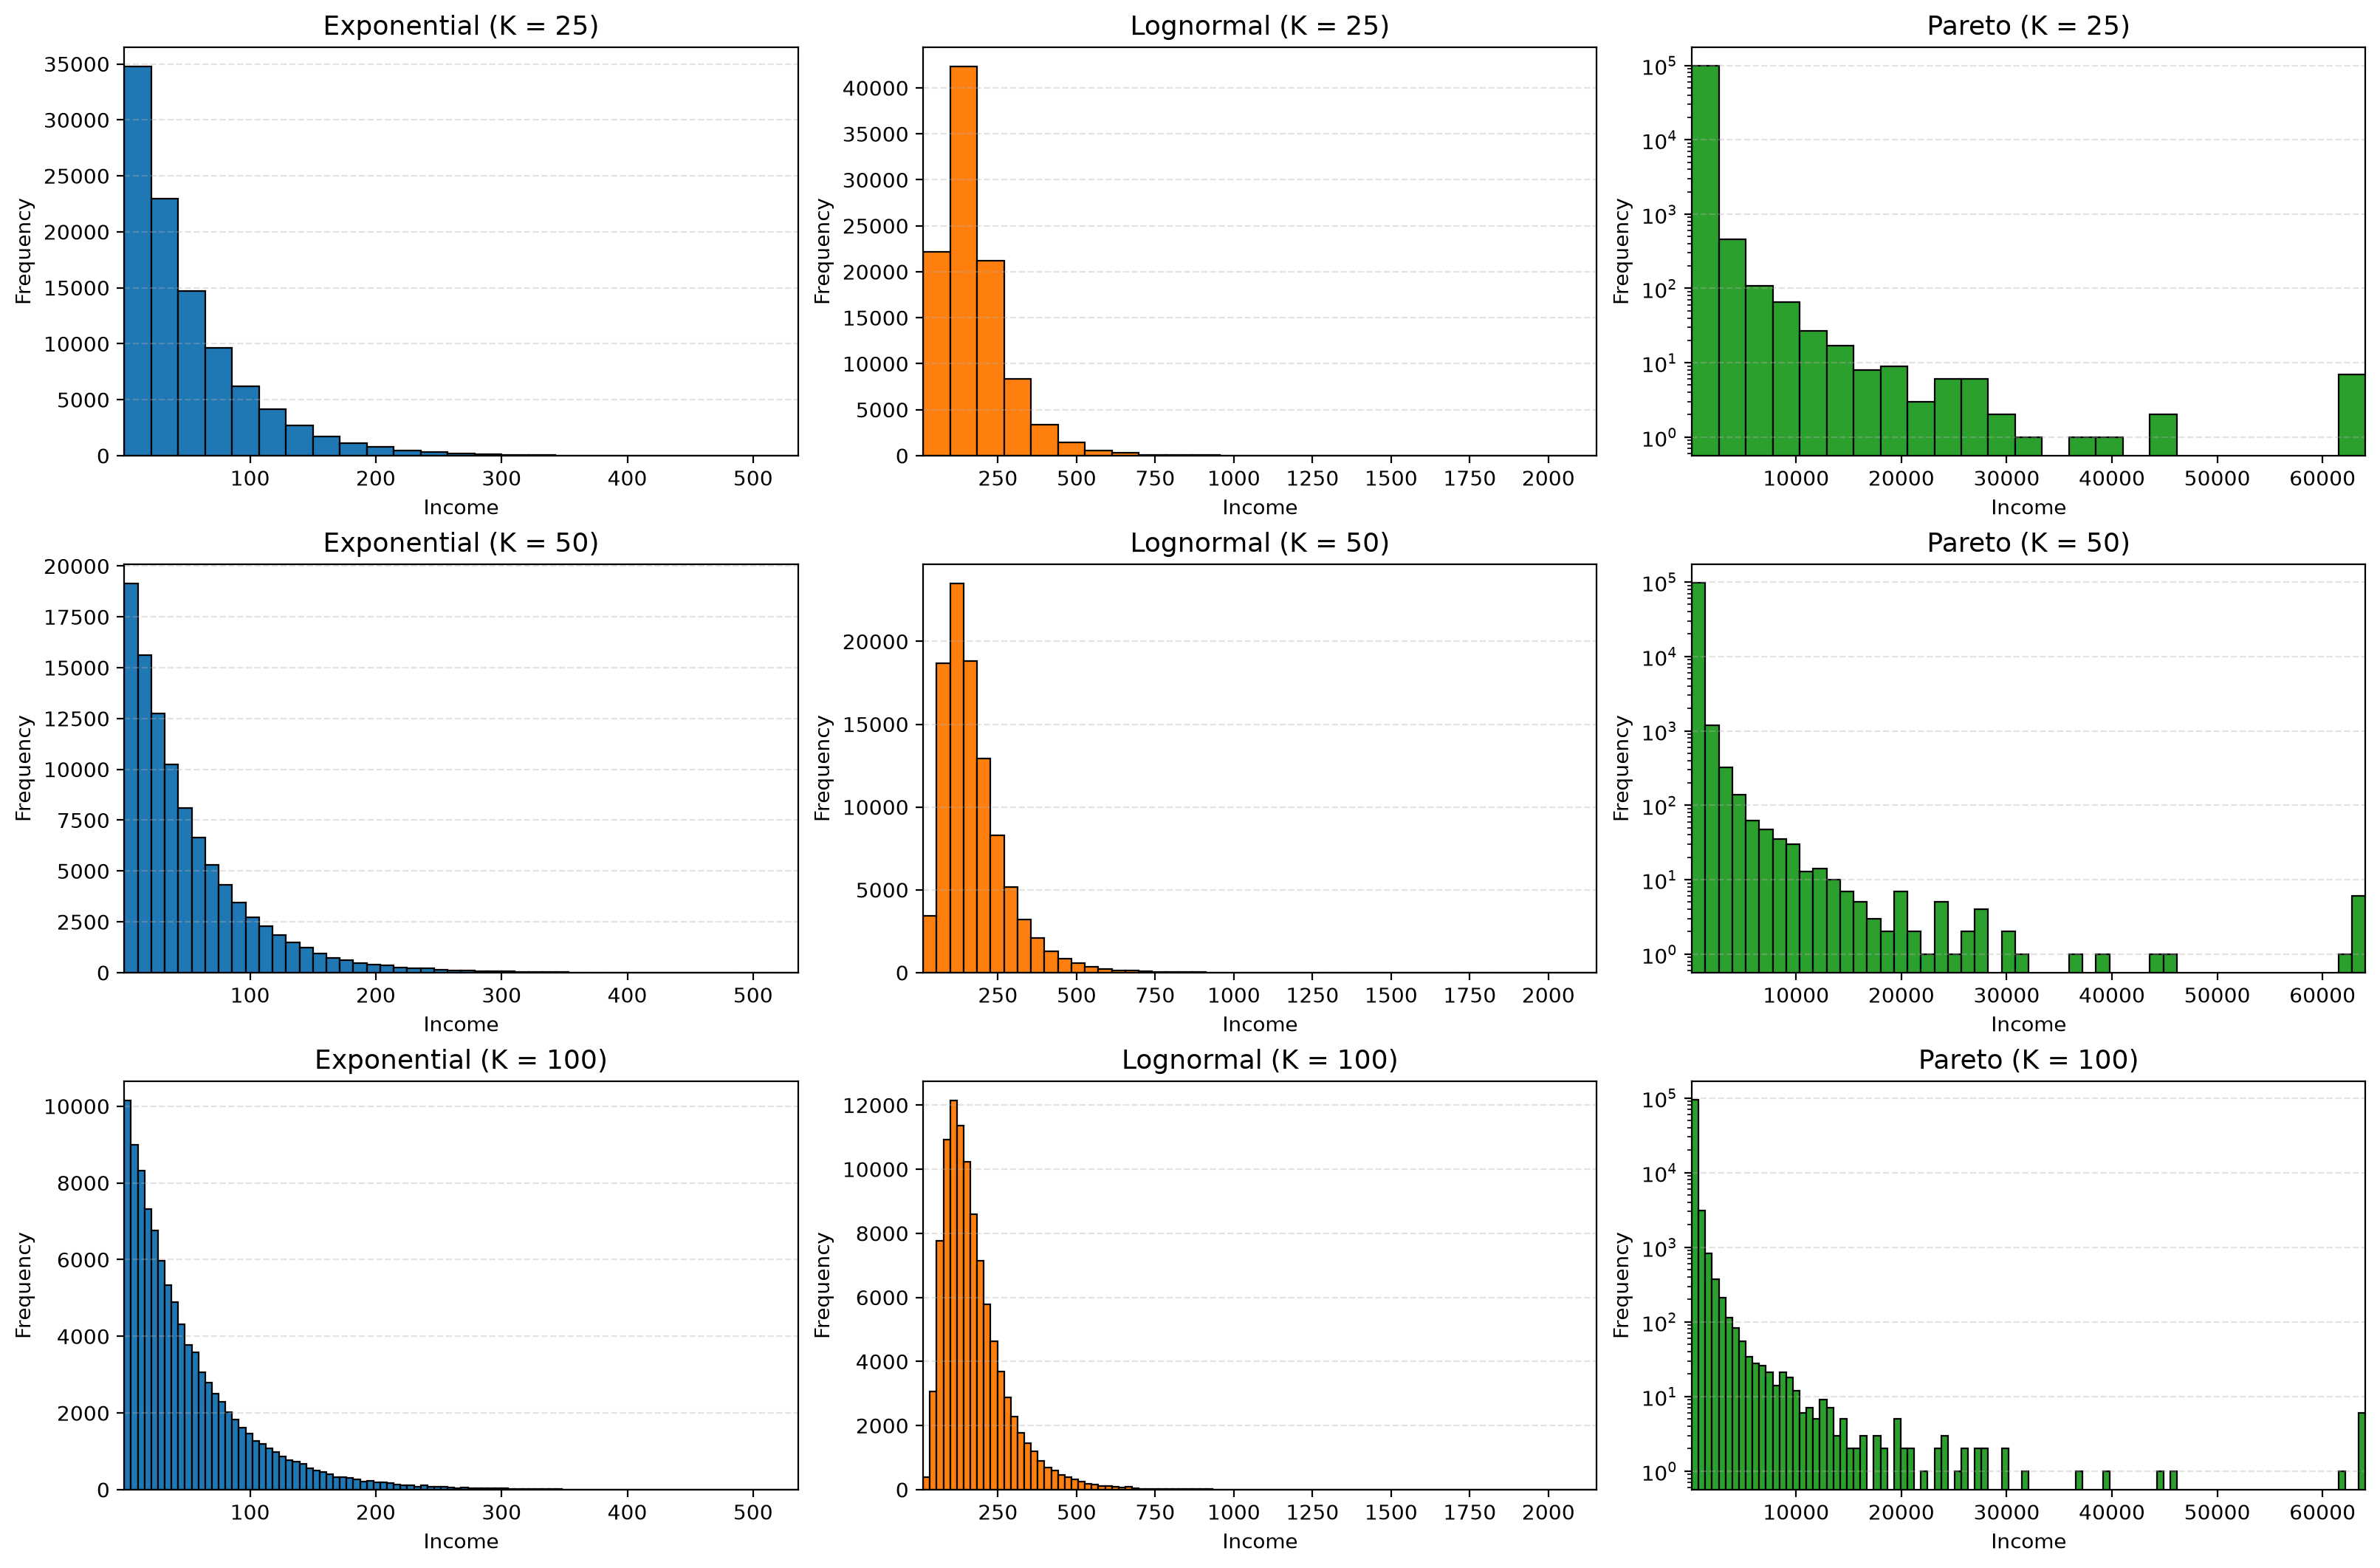
\includegraphics[width=0.92\textwidth]{histograms.png}
\caption{Synthetic exponential, lognormal, and Pareto samples represented with ordinary equal-width histograms for $K=25$, $50$, and $100$ bins. The Pareto panels retain a logarithmic vertical scale and a conservative visual truncation of only the most extreme observations. The same distributional parameters and random seed are used throughout the numerical comparison.}
\label{fig:synthetic-histograms}
\end{figure}

Figure~\ref{fig:synthetic-histograms} already displays the essential difficulty. The exponential and lognormal samples have ranges that remain manageable under ordinary binning. The Pareto sample, by contrast, develops a long sparse tail whose statistical structure is difficult to display with a fixed linear horizontal scale.

\subsection{Exponential, lognormal, and Pareto distributions}

The three laws used here differ fundamentally in their asymptotic decay. The exponential law possesses a characteristic scale and suppresses very large events exponentially. The lognormal law is broader and arises naturally from multiplicative mechanisms. The Pareto law has no exponential cutoff and assigns substantially more probability to extreme values. Standard probability references such as Ross \cite{Ross2014} provide the basic theory; the lognormal distribution and its empirical ubiquity are reviewed in detail by Limpert, Stahel, and Abbt \cite{LimpertStahelAbbt2001}.

\begin{definition}[Exponential distribution]
A nonnegative random variable $X$ is exponentially distributed with rate $\lambda>0$, written $X\sim\mathrm{Exp}(\lambda)$, if its probability density is
\begin{equation}
 f_X(x)=
 \begin{cases}
 \lambda e^{-\lambda x}, & x\geq 0,\\
 0, & x<0.
 \end{cases}
\end{equation}
Its cumulative and complementary cumulative distribution functions are
\begin{align}
 F_X(x) &= 1-e^{-\lambda x},\\
 \overline F_X(x) &= e^{-\lambda x},
\end{align}
for $x\geq 0$, and its first two moments are
\begin{equation}
 \mathbb{E}[X]=\frac{1}{\lambda},
 \qquad
 \mathrm{Var}(X)=\frac{1}{\lambda^2}.
\end{equation}
\end{definition}

The exponential law is the canonical waiting-time distribution of a homogeneous Poisson process. If events occur independently at constant rate $\lambda$, then the time between consecutive events is exponentially distributed. This makes the law a natural light-tailed benchmark: the probability of an observation larger than $x$ is suppressed as $e^{-\lambda x}$. In the binning experiments, this rapid decay gives a reference case in which the maximum grows slowly enough that ordinary equal-width intervals remain reasonably informative.

A broader distribution is obtained when randomness acts multiplicatively rather than additively. Taking logarithms converts products into sums, so repeated independent multiplicative factors naturally motivate a Gaussian approximation in log space. This leads to the next model.

\begin{definition}[Lognormal distribution]
A positive random variable $X$ is lognormally distributed with parameters $\mu\in\R$ and $\sigma>0$, written $X\sim\mathrm{Lognormal}(\mu,\sigma^2)$, if $Y=\ln X$ is normally distributed with mean $\mu$ and variance $\sigma^2$. Its density is
\begin{equation}
 f_X(x)=\frac{1}{x\sigma\sqrt{2\pi}}
 \exp\left[-\frac{(\ln x-\mu)^2}{2\sigma^2}\right],
 \qquad x>0.
\end{equation}
Its mean and variance are
\begin{align}
 \mathbb{E}[X] &= \exp\left(\mu+\frac{\sigma^2}{2}\right),\\
 \mathrm{Var}(X) &= \left(e^{\sigma^2}-1\right)e^{2\mu+\sigma^2}.
\end{align}
\end{definition}

The lognormal distribution is associated with multiplicative random mechanisms: products of many independent positive random factors become sums after taking logarithms, so a central-limit argument can produce approximate normality in log space. Newman \cite{Newman2005} explicitly discusses the lognormal law as an important broad-tailed alternative that can mimic power-law behavior over a finite range. This observation is methodologically important because apparent linearity over a short log--log interval does not uniquely identify a Pareto tail. Its moments are finite for every finite order, but its right tail is substantially broader than an exponential tail, which makes it a useful intermediate case between light-tailed and genuinely scale-free behavior.

The Pareto family changes the asymptotic regime qualitatively. Instead of exponential or lognormal suppression, probability decreases algebraically, so extreme observations remain much more frequent and the existence of moments depends directly on the tail exponent.

\begin{definition}[Pareto or continuous power-law distribution]
Let $x_{\min}>0$ and $\alpha>1$. A positive random variable $X$ follows the continuous power-law distribution used in these notes if
\begin{equation}
 f_X(x)=
 \begin{cases}
 (\alpha-1)x_{\min}^{\alpha-1}x^{-\alpha}, & x\geq x_{\min},\\
 0, & x<x_{\min}.
 \end{cases}
\label{eq:pareto-pdf}
\end{equation}
The corresponding complementary cumulative distribution is
\begin{equation}
 \overline F_X(x)=\mathbb{P}(X>x)
 =\left(\frac{x}{x_{\min}}\right)^{-(\alpha-1)},
 \qquad x\geq x_{\min}.
\label{eq:pareto-ccdf}
\end{equation}
\end{definition}

This notation follows Newman \cite{Newman2005}: $\alpha$ denotes the exponent of the probability density. In the common Pareto Type-I parameterization the shape parameter is instead $k=\alpha-1$. The distinction matters because the CCDF exponent is one unit smaller than the PDF exponent. Pareto's original work on income concentration provides the historical origin of this family \cite{Pareto1896}. The algebraic tail also implies that moment existence cannot be assumed automatically; it must be checked from the exponent.

\begin{proposition}[Existence of Pareto moments]
For the density in Eq.~\eqref{eq:pareto-pdf}, the moment $\mathbb{E}[X^m]$ is finite if and only if $\alpha>m+1$.
\end{proposition}

\begin{demonstration}
For $m\geq0$,
\begin{align}
\mathbb{E}[X^m]
&=(\alpha-1)x_{\min}^{\alpha-1}
\int_{x_{\min}}^{\infty}x^{m-\alpha}\,\dd x.
\end{align}
The improper integral converges precisely when $m-\alpha<-1$, equivalently when $\alpha>m+1$. Therefore the mean requires $\alpha>2$, while the variance requires $\alpha>3$.
\end{demonstration}

For the synthetic value $\alpha=2.5$, the theoretical mean exists but the variance diverges. Large observations are therefore not incidental anomalies; they are intrinsic to the model and strongly influence finite-sample summaries. This is one reason why a heavy-tail visualization should not be designed by simply suppressing the observations that make the plot inconvenient.

\subsection{Statistical distributions, PDF, CDF, and CCDF}

The preceding examples can be placed in a common measure-theoretic framework. The basic object is not a formula for a density but the probability law induced by a random variable. Densities, cumulative probabilities, and survival probabilities are alternative representations of that same law when the necessary regularity conditions hold.

\begin{definition}[Distribution of a random variable]
Let $(\Omega,\mathcal{F},\mathbb{P})$ be a probability space and let $X:\Omega\rightarrow\R$ be a measurable random variable. The distribution of $X$ is the probability measure $\mathbb{P}_X$ on the Borel sets of $\R$ defined by
\begin{equation}
 \mathbb{P}_X(A)=\mathbb{P}(X\in A),
 \qquad A\in\mathcal{B}(\R).
\end{equation}
\end{definition}

The distribution therefore assigns probability to measurable subsets of the state space. For continuous models it is often convenient to express this measure through a density, but the density itself should not be confused with a probability: it has units inverse to those of $X$, and probabilities are obtained only after integration over an interval.

\begin{definition}[Probability density function]
If $\mathbb{P}_X$ is absolutely continuous with respect to Lebesgue measure, then there exists a nonnegative function $f_X$ such that
\begin{equation}
 \mathbb{P}(a<X\leq b)=\int_a^b f_X(t)\,\dd t,
\end{equation}
with
\begin{equation}
 \int_{-\infty}^{\infty} f_X(t)\,\dd t=1.
\end{equation}
The function $f_X$ is the probability density function, or PDF.
\end{definition}

The density is local: it describes how rapidly probability accumulates per unit change in the variable. Cumulative representations instead collect probability from one side of the real line and are therefore naturally monotone. This distinction becomes useful in heavy-tail analysis because cumulative objects do not require a preliminary choice of bins.

\begin{definition}[Cumulative distribution function]
The cumulative distribution function of $X$ is
\begin{equation}
 F_X(x)=\mathbb{P}(X\leq x).
\end{equation}
For an absolutely continuous distribution,
\begin{equation}
 F_X(x)=\int_{-\infty}^{x}f_X(t)\,\dd t.
\end{equation}
\end{definition}

The CDF measures the probability accumulated to the left of $x$. In tail problems the complementary quantity is often more transparent because it directly reports the probability of exceeding a threshold and can be read as a survival probability.

\begin{definition}[Complementary cumulative distribution function]
The complementary cumulative distribution function, also called the survival function, is
\begin{equation}
 \overline F_X(x)=1-F_X(x)=\mathbb{P}(X>x).
\label{eq:ccdf-general}
\end{equation}
For continuous $X$, replacing $X>x$ by $X\geq x$ does not change the probability.
\end{definition}

The distinction between a density and a cumulative probability is essential. A PDF describes probability per unit $x$ and therefore must be normalized by bin width when estimated with a histogram whose widths vary. A CDF or CCDF is dimensionless and does not require binning. For heavy-tailed data this makes the empirical CCDF especially attractive: every observation can contribute directly to the curve without a preliminary choice of histogram edges. Newman \cite{Newman2005} uses this property to motivate cumulative and rank-frequency representations, while Clauset, Shalizi, and Newman \cite{ClausetShaliziNewman2009} emphasize that graphical agreement remains only exploratory evidence and not a goodness-of-fit test.

For a sample $x_1,\ldots,x_n$, the empirical CDF and CCDF are
\begin{align}
 \widehat F_n(x)
 &=\frac{1}{n}\sum_{i=1}^{n}\mathbf{1}_{\{x_i\leq x\}},\\
 \widehat{\overline F}_n(x)
 &=\frac{1}{n}\sum_{i=1}^{n}\mathbf{1}_{\{x_i>x\}}.
\end{align}
They are step functions defined directly from the ordered sample. This absence of bin boundaries is one reason the empirical CCDF is particularly useful as a companion to histogram-based diagnostics.

\subsection{Practical examples and empirical data sources}

Broad distributions occur in many disciplines, but the word ``power law'' should be reserved for a statistical statement supported by an explicit tail model rather than by visual resemblance alone. Table~\ref{tab:empirical-examples} summarizes several data sets discussed by Newman \cite{Newman2005}, together with the sources from which those data were obtained, and includes the Brazilian income application of Moura Jr. and Ribeiro \cite{MouraRibeiro2009}.

\begin{table}[htbp]
\centering
\caption{Examples of broad or power-law-like empirical distributions and the corresponding data sources.}
\label{tab:empirical-examples}
\begin{adjustbox}{max width=\textwidth}
\begin{tabular}{p{0.22\textwidth}p{0.33\textwidth}p{0.35\textwidth}}
\toprule
Quantity & Empirical context & Source and reference \\
\midrule
Brazilian personal income & Brazilian personal-income samples, 1978--2005; the upper-income component was modeled with a Pareto tail & Moura Jr. and Ribeiro \cite{MouraRibeiro2009} \\
\addlinespace[0.45em]
US city populations & City populations from the 2000 Census; upper-range behavior discussed as a power-law example & U.S. Census Bureau \cite{USCensus2000}; analysis in Newman \cite{Newman2005} \\
\addlinespace[0.45em]
California earthquakes & Earthquakes from January 1910 to May 1992 in the Berkeley Earthquake Catalog & National Geophysical Data Center \cite{NOAANGDC}; discussion in Newman \cite{Newman2005} \\
\addlinespace[0.45em]
Solar-flare peak intensity & Hard X-Ray Burst Spectrometer observations aboard the Solar Maximum Mission, 1980--1989 & NASA Goddard Space Flight Center \cite{NASASMM}; physical discussion by Lu and Hamilton \cite{LuHamilton1991}; compilation in Newman \cite{Newman2005} \\
\addlinespace[0.45em]
Wealth of richest Americans & Aggregate net worth of the richest U.S. individuals in October 2003 & Forbes 400 data \cite{Forbes2003}; analysis in Newman \cite{Newman2005} \\
\bottomrule
\end{tabular}
\end{adjustbox}
\end{table}

The examples illustrate why tail resolution is a substantive issue rather than a cosmetic one. In earthquake or flare data, the tail contains rare high-impact events; in city-size and wealth data, it contains the largest systems or fortunes; and in income data it contains a small fraction of observations with disproportionate economic weight. A representation that leaves the tail with one or two noisy bins discards precisely the part of the sample that often motivates the analysis.



\section{Binning methods}

This section turns from probability models to discretization. We first define binning as a partition of the data domain and briefly review classical rules for choosing the number or width of histogram bins. We then study the three constructions used in the numerical experiments: quantile binning through \texttt{pandas.qcut}, equal-width binning through \texttt{pandas.cut}, and logarithmic binning through geometrically spaced edges. The main analytical result is that, after the essential normalization by bin width, logarithmic binning preserves the exponent of an ideal power-law density while allocating increasingly wide intervals to the sparsely populated tail.

\subsection{What binning is and why there are several strategies}

\begin{definition}[Binning]
Let $I\subseteq\R$ be an interval containing the observed data. A binning of $I$ is a finite ordered partition
\begin{equation}
 I=B_1\cup B_2\cup\cdots\cup B_K,
 \qquad B_j\cap B_k=\varnothing\quad(j\neq k),
\label{eq:partition}
\end{equation}
up to a fixed convention for observations that fall exactly on shared boundaries.
\end{definition}

Equation~\eqref{eq:partition} separates the data domain into mutually exclusive classes whose union recovers the working interval. Membership can be represented compactly by an indicator operator, which is useful both mathematically and computationally.

\begin{definition}[Indicator function]
For a set $A\subseteq\R$, the indicator of $A$ is the function $\mathbf{1}_A:\R\rightarrow\{0,1\}$ defined by
\[
\mathbf{1}_A(x)=
\begin{cases}
1, & x\in A,\\
0, & x\notin A.
\end{cases}
\]
Thus $\mathbf{1}_{B_k}(x_i)$ records whether observation $x_i$ belongs to the $k$th bin.
\end{definition}

For a sample $x_1,\ldots,x_n$, bin occupancy and conservation of the total sample size are then expressed by the paired relations
\begin{subequations}\label{eq:occupancy}
\begin{align}
 n_k &= \sum_{i=1}^{n}\mathbf{1}_{B_k}(x_i),
 \label{eq:occupancy-a}\\
 \sum_{k=1}^{K} n_k &= n.
 \label{eq:occupancy-b}
\end{align}
\end{subequations}
Equation~\eqref{eq:occupancy-a} states that the occupancy $n_k$ is obtained by adding one unit for every observation that belongs to $B_k$ and zero otherwise. Equation~\eqref{eq:occupancy-b} follows from the fact that the bins form a partition: every observation is assigned to exactly one bin, so summing occupancies over all bins recovers the full sample size.

Table~\ref{tab:toy-binning} gives a minimal data set in which the bin name is made explicit. The deliberately skewed values illustrate why the partition geometry matters even before a histogram is drawn.

\begin{table}[htbp]
\centering
\caption{Toy data set assigned to four equal-width bins over the interval $[0,100]$.}
\label{tab:toy-binning}
\begin{tabular}{rrl}
\toprule
Observation & Value $x_i$ & Bin name \\
\midrule
1 & 2.0 & $B_1=[0,25)$ \\
2 & 3.0 & $B_1=[0,25)$ \\
3 & 3.5 & $B_1=[0,25)$ \\
4 & 4.0 & $B_1=[0,25)$ \\
5 & 5.0 & $B_1=[0,25)$ \\
6 & 6.0 & $B_1=[0,25)$ \\
7 & 8.0 & $B_1=[0,25)$ \\
8 & 10.0 & $B_1=[0,25)$ \\
9 & 14.0 & $B_1=[0,25)$ \\
10 & 20.0 & $B_1=[0,25)$ \\
11 & 40.0 & $B_2=[25,50)$ \\
12 & 100.0 & $B_4=[75,100]$ \\
\bottomrule
\end{tabular}
\end{table}

\begin{figure}[!htbp]
\centering
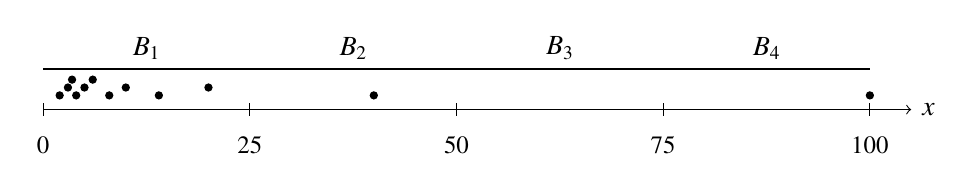
\begin{tikzpicture}[x=0.105cm,y=1cm]
\draw[->] (0,0) -- (105,0) node[right] {$x$};
\foreach \x in {0,25,50,75,100}{\draw (\x,0.08)--(\x,-0.08) node[below=4pt]{\small \x};}
\draw[thick] (0,0.52)--(25,0.52);
\draw[thick] (25,0.52)--(50,0.52);
\draw[thick] (50,0.52)--(75,0.52);
\draw[thick] (75,0.52)--(100,0.52);
\node at (12.5,0.78) {$B_1$};
\node at (37.5,0.78) {$B_2$};
\node at (62.5,0.78) {$B_3$};
\node at (87.5,0.78) {$B_4$};
\foreach \x/\y in {2/0.18,3/0.28,3.5/0.38,4/0.18,5/0.28,6/0.38,8/0.18,10/0.28,14/0.18,20/0.28,40/0.18,100/0.18}{\fill (\x,\y) circle (1.5pt);}
\end{tikzpicture}
\caption{Illustrative equal-width partition of the toy sample in Table~\ref{tab:toy-binning}. Most observations occupy the first interval, the third interval is empty, and the largest observation determines the full linear range.}
\label{fig:toy-binning}
\end{figure}

A histogram supplements the partition with a vertical statistic. For equal-width bins, raw counts or relative frequencies are directly comparable because all intervals have the same width. For unequal-width bins, raw counts confound local probability mass with geometric interval size. A density histogram therefore uses
\begin{equation}
 \widehat f_k=\frac{n_k}{n\,\Delta_k},
 \qquad
 \Delta_k=b_{k+1}-b_k,
\label{eq:density-hist}
\end{equation}
where $b_k$ and $b_{k+1}$ are consecutive bin edges. This normalization guarantees
\begin{equation}
 \sum_{k=1}^{K}\widehat f_k\Delta_k=1.
\end{equation}

There is no universal optimal partition. Sturges \cite{Sturges1926} proposed a classical rule for the number of classes; Scott \cite{Scott1979} derived an asymptotically motivated bandwidth for density estimation; and Freedman and Diaconis \cite{FreedmanDiaconis1981} proposed a robust width proportional to the interquartile range and $n^{-1/3}$. Adaptive strategies also exist. Bayesian Blocks chooses change points by optimizing a statistical fitness function rather than prescribing a constant width \cite{ScargleEtAl2013}, while kernel density estimation replaces hard intervals by smooth local kernels. These methods are useful context, but the present notes focus on three transparent partitions whose geometry can be inspected directly.

The first is equal-width binning: each interval has the same length in the original coordinate. The second is quantile binning: the interval boundaries are empirical quantiles, so occupancies are approximately equal and widths adapt to the local density of observations. The third is logarithmic binning: bin edges are equally spaced after taking logarithms, which means that widths increase geometrically in the original variable. The three choices therefore equalize different objects---width in $x$, probability mass, and width in $\log x$, respectively.

\subsection{Quantile binning with \texttt{pandas.qcut}}

The pandas function \texttt{qcut} implements quantile-based discretization \cite{PandasQcut}. For an integer $K$, it attempts to divide a one-dimensional sample into $K$ groups with equal or nearly equal numbers of observations. Unlike equal-width binning, the geometry is determined by the empirical distribution itself: dense regions receive narrow intervals, while sparse regions receive broad intervals.

\begin{definition}[Empirical quantile]
For observations $x_1,\ldots,x_n$, define the empirical CDF $\widehat F_n$. For $p\in(0,1)$, an empirical quantile can be defined by
\begin{equation}
 \widehat Q_n(p)=\inf\left\{x:\widehat F_n(x)\geq p\right\}.
\end{equation}
A $K$-quantile partition uses the edges
\begin{equation}
 b_k=\widehat Q_n\left(\frac{k}{K}\right),
 \qquad k=0,1,\ldots,K,
\end{equation}
with endpoint conventions chosen to include the sample minimum and maximum.
\end{definition}

The definition makes clear that equal probability content, rather than equal geometric width, is the organizing principle. When the sample is continuous and ties are absent, rank information gives an especially simple occupancy result.

\begin{proposition}[Occupancy of quantile bins]
If the sample has no ties at the chosen quantile boundaries and $K$ divides $n$, an exact rank-based $K$-quantile partition contains $n/K$ observations in every bin.
\end{proposition}

\begin{demonstration}
Order the sample as $x_{(1)}<\cdots<x_{(n)}$. If $K$ divides $n$, define boundaries after the ranks $n/K,2n/K,\ldots,(K-1)n/K$. Each consecutive block then contains exactly $n/K$ order statistics. The absence of ties guarantees that no observation is ambiguous at a shared boundary.
\end{demonstration}

This is the defining practical advantage of \texttt{qcut}: statistical summaries computed inside different bins are based on comparable sample sizes. The method is therefore useful for income deciles, score quintiles, credit-risk bands, or any application in which balanced groups are more important than fixed numerical widths. Its limitation is equally clear: consecutive bins no longer correspond to equal changes in the measured variable, so the physical interpretation of a one-bin displacement varies across the distribution.

For the toy sample used in Sec.~3.1, quartile binning is implemented by
\begin{lstlisting}[caption={Quartile binning with pandas.qcut.}]
import pandas as pd

x = [2, 3, 3.5, 4, 5, 6, 8, 10, 14, 20, 40, 100]
labels, edges = pd.qcut(
    x,
    q=4,
    labels=False,
    retbins=True,
    duplicates="raise",
)
print(edges)
print(labels.to_numpy())
\end{lstlisting}
The corresponding output is
\begin{lstlisting}[caption={Output of the quartile example.},numbers=none]
[  2.      3.875   7.     15.5   100.   ]
[0 0 0 1 1 1 2 2 2 3 3 3]
\end{lstlisting}

Table~\ref{tab:qcut-example} displays the same result as named quartile bins. The widths increase from $1.875$ in the first quartile to $84.5$ in the fourth, while the occupancy remains exactly three observations per bin.

\begin{table}[htbp]
\centering
\caption{Quartile assignment returned by \texttt{qcut} for the toy sample.}
\label{tab:qcut-example}
\begin{tabular}{lll}
\toprule
Values & Bin name & Interval determined by empirical quantiles \\
\midrule
$2,3,3.5$ & $Q_1$ & $[2,3.875]$ \\
$4,5,6$ & $Q_2$ & $(3.875,7]$ \\
$8,10,14$ & $Q_3$ & $(7,15.5]$ \\
$20,40,100$ & $Q_4$ & $(15.5,100]$ \\
\bottomrule
\end{tabular}
\end{table}

In applied data, duplicate quantile edges can arise when many observations share the same value. The pandas implementation allows the user either to raise an error or to remove non-unique edges through the \texttt{duplicates} argument \cite{PandasQcut}. This behavior should be treated as a substantive feature of discrete or rounded data rather than as a purely technical nuisance, because dropping an edge changes the intended number of groups.

\subsection{Equal-width binning with \texttt{pandas.cut}}

The function \texttt{cut} discretizes values according to explicit interval boundaries or, when the number of bins is supplied as an integer, according to equal-width intervals over the observed range \cite{PandasCut}. Its geometry is therefore defined in the original measurement scale. If the working interval is $[a,b]$ and $K$ equal bins are required, the idealized edges are
\begin{equation}
 b_k=a+k\Delta,
 \qquad
 \Delta=\frac{b-a}{K},
 \qquad
 k=0,1,\ldots,K.
\label{eq:cut-edges}
\end{equation}

This construction is natural when additive differences in the original unit are physically meaningful. Age bands of five years, temperature intervals of two degrees, and laboratory measurements reported on a fixed linear scale are typical examples. Equal widths also make raw counts directly comparable because every interval represents the same amount of the underlying variable.

The weakness of the method is its dependence on the total observed range $b-a$. A single extreme observation can enlarge every interval simultaneously, reducing resolution where most observations are concentrated. The toy sample already contains this mechanism: the observation $x=100$ makes a four-bin linear partition much coarser than the quartile partition of the same twelve values.

Using four bins for direct comparison with the \texttt{qcut} example,
\begin{lstlisting}[caption={Equal-width binning with pandas.cut.}]
import pandas as pd

x = [2, 3, 3.5, 4, 5, 6, 8, 10, 14, 20, 40, 100]
labels, edges = pd.cut(
    x,
    bins=4,
    labels=False,
    retbins=True,
    include_lowest=True,
)
print(edges)
print(labels.to_numpy())
\end{lstlisting}
produces
\begin{lstlisting}[caption={Output of the equal-width example.},numbers=none]
[  1.902  26.5    51.     75.5   100.   ]
[0 0 0 0 0 0 0 0 0 0 1 3]
\end{lstlisting}

The first edge is slightly below the observed minimum because pandas extends the range by $0.1\%$ when an integer number of bins is supplied, thereby ensuring that the minimum and maximum are included \cite{PandasCut}. Table~\ref{tab:cut-example} shows the resulting occupancy structure.

\begin{table}[htbp]
\centering
\caption{Equal-width assignment returned by \texttt{cut} for the toy sample.}
\label{tab:cut-example}
\begin{tabular}{lll}
\toprule
Values & Bin name & Interval \\
\midrule
$2,3,3.5,4,5,6,8,10,14,20$ & $B_1$ & $[1.902,26.5]$ \\
$40$ & $B_2$ & $(26.5,51]$ \\
--- & $B_3$ & $(51,75.5]$ \\
$100$ & $B_4$ & $(75.5,100]$ \\
\bottomrule
\end{tabular}
\end{table}

The comparison with Table~\ref{tab:qcut-example} isolates the central distinction. \texttt{qcut} adapts widths to obtain balanced occupancies, whereas \texttt{cut} holds widths approximately fixed and allows occupancies to vary. For broad or heavy-tailed samples the latter variation can be extreme, and Sec.~4 quantifies this effect for the synthetic Pareto experiment.

\subsection{Logarithmic binning}

Logarithmic binning is designed for strictly positive variables whose dynamic range is naturally multiplicative. The method appears prominently in Newman's treatment of power-law data, where ordinary fixed-width histograms become increasingly noisy in the tail because the expected number of observations per bin decreases rapidly \cite{Newman2005}. The same principle has been advocated in other empirical domains, including information science, as a way to aggregate sparse tail observations without discarding the multiplicative structure of the data \cite{Milojevic2010}. More generally, analysis of binned power-law data requires explicit attention to the information lost through aggregation, a point developed statistically by Virkar and Clauset \cite{VirkarClauset2014}.

The construction replaces constant additive increments by constant multiplicative increments. In log coordinates the edges are equally spaced; after transforming back to the original variable, the intervals widen geometrically.

\begin{definition}[Logarithmic binning]
Let $0<x_{\min}<x_{\max}$ and let $K\in\N$. Define
\begin{equation}
 r=\left(\frac{x_{\max}}{x_{\min}}\right)^{1/K}>1.
\end{equation}
The logarithmic bin edges are
\begin{equation}
 b_k=x_{\min}r^k,
 \qquad k=0,1,\ldots,K.
\label{eq:log-edges}
\end{equation}
Equivalently, $\log b_k$ is an arithmetic progression.
\end{definition}

The ratio $r$ controls multiplicative resolution: increasing the bin index by one multiplies the edge by the same factor everywhere in the domain. The width of the $k$th bin is
\begin{equation}
 \Delta_k=b_{k+1}-b_k=(r-1)b_k,
\label{eq:log-width}
\end{equation}
so the absolute width grows linearly with the lower edge. A convenient representative horizontal coordinate is the geometric center
\begin{equation}
 c_k=\sqrt{b_kb_{k+1}}=b_k\sqrt{r},
\end{equation}
which is the midpoint in logarithmic coordinates. This choice respects the same multiplicative geometry that defines the bins.

The widening of the intervals is not an arbitrary smoothing device. In a decreasing heavy-tailed distribution, expected counts per unit linear width become very small at large $x$. Aggregating a wider range in the tail partially compensates for that loss of observations and reduces the visual variance of the empirical histogram. The price is reduced local resolution: binning always discards within-bin information, and excessive logarithmic aggregation can hide curvature, cutoffs, or crossovers. Virkar and Clauset \cite{VirkarClauset2014} quantify this general loss of statistical power for binned power-law data, reinforcing the distinction between a useful visualization and a formal inferential procedure.

A second issue is normalization. Because $\Delta_k$ varies strongly with $k$, raw counts or raw relative frequencies cannot be interpreted as estimates of a common density scale. If the objective is to estimate a PDF, the appropriate histogram height is the width-normalized quantity in Eq.~\eqref{eq:density-hist}. Newman \cite{Newman2005} stresses this correction in logarithmically binned power-law plots, and the following result makes the reason explicit.

\begin{theorem}[Power-law exponent under logarithmic binning]
Suppose $X$ has density $f(x)=Cx^{-\alpha}$ on a range covered by logarithmic bins $[b_k,b_{k+1})$ with $b_{k+1}=rb_k$, where $r>1$ and $\alpha>1$. Then the expected density-histogram height in bin $k$ is proportional to $b_k^{-\alpha}$. Hence the logarithmic-bin density preserves the PDF exponent $\alpha$.
\end{theorem}

\begin{demonstration}
The probability mass of bin $k$ is
\begin{align}
 p_k
 &=\int_{b_k}^{rb_k}Cx^{-\alpha}\,\dd x\\
 &=\frac{C}{\alpha-1}
 \left(b_k^{1-\alpha}-(rb_k)^{1-\alpha}\right)\\
 &=\frac{C}{\alpha-1}
 \left(1-r^{1-\alpha}\right)b_k^{1-\alpha}.
\end{align}
Using Eq.~\eqref{eq:log-width}, the corresponding probability per unit width is
\begin{align}
 \frac{p_k}{\Delta_k}
 &=\frac{C}{(\alpha-1)(r-1)}
 \left(1-r^{1-\alpha}\right)b_k^{-\alpha}.
\end{align}
All factors except $b_k^{-\alpha}$ are constant across bins. Therefore the expected density histogram has the same power-law exponent as the underlying PDF.
\end{demonstration}

The theorem also explains a common plotting error. If logarithmic-bin probabilities $p_k$ are plotted without division by $\Delta_k$, they scale as $b_k^{1-\alpha}$ rather than $b_k^{-\alpha}$, shifting the apparent slope by one. Width normalization is therefore a mathematical requirement for density estimation, not a cosmetic convention. Even after this correction, however, exponent estimation should not be reduced to a straight-line fit on a log--log graph. Maximum-likelihood estimation, explicit treatment of the lower cutoff, goodness-of-fit testing, and comparison with alternative heavy-tailed models remain necessary for empirical inference \cite{ClausetShaliziNewman2009,VirkarClauset2014}.

Figure~\ref{fig:newman-grid} follows the pedagogical logic of Newman \cite{Newman2005} with an independently generated sample of $10^6$ Pareto observations having $\alpha=2.5$. Panel (a) shows the distribution on linear axes, where the tail is visually compressed. Panel (b) uses logarithmic coordinates with fixed linear-width aggregation and exposes the approximate power-law trend, but the far tail becomes noisy because counts become small. Panel (c) uses logarithmically widening bins and width normalization, reducing this heteroscedastic tail noise while preserving the theoretical power-law exponent. Panel (d) shows the empirical CCDF, which avoids histogram boundaries and supplies a complementary view of the same tail.

\begin{figure}[!htbp]
\centering
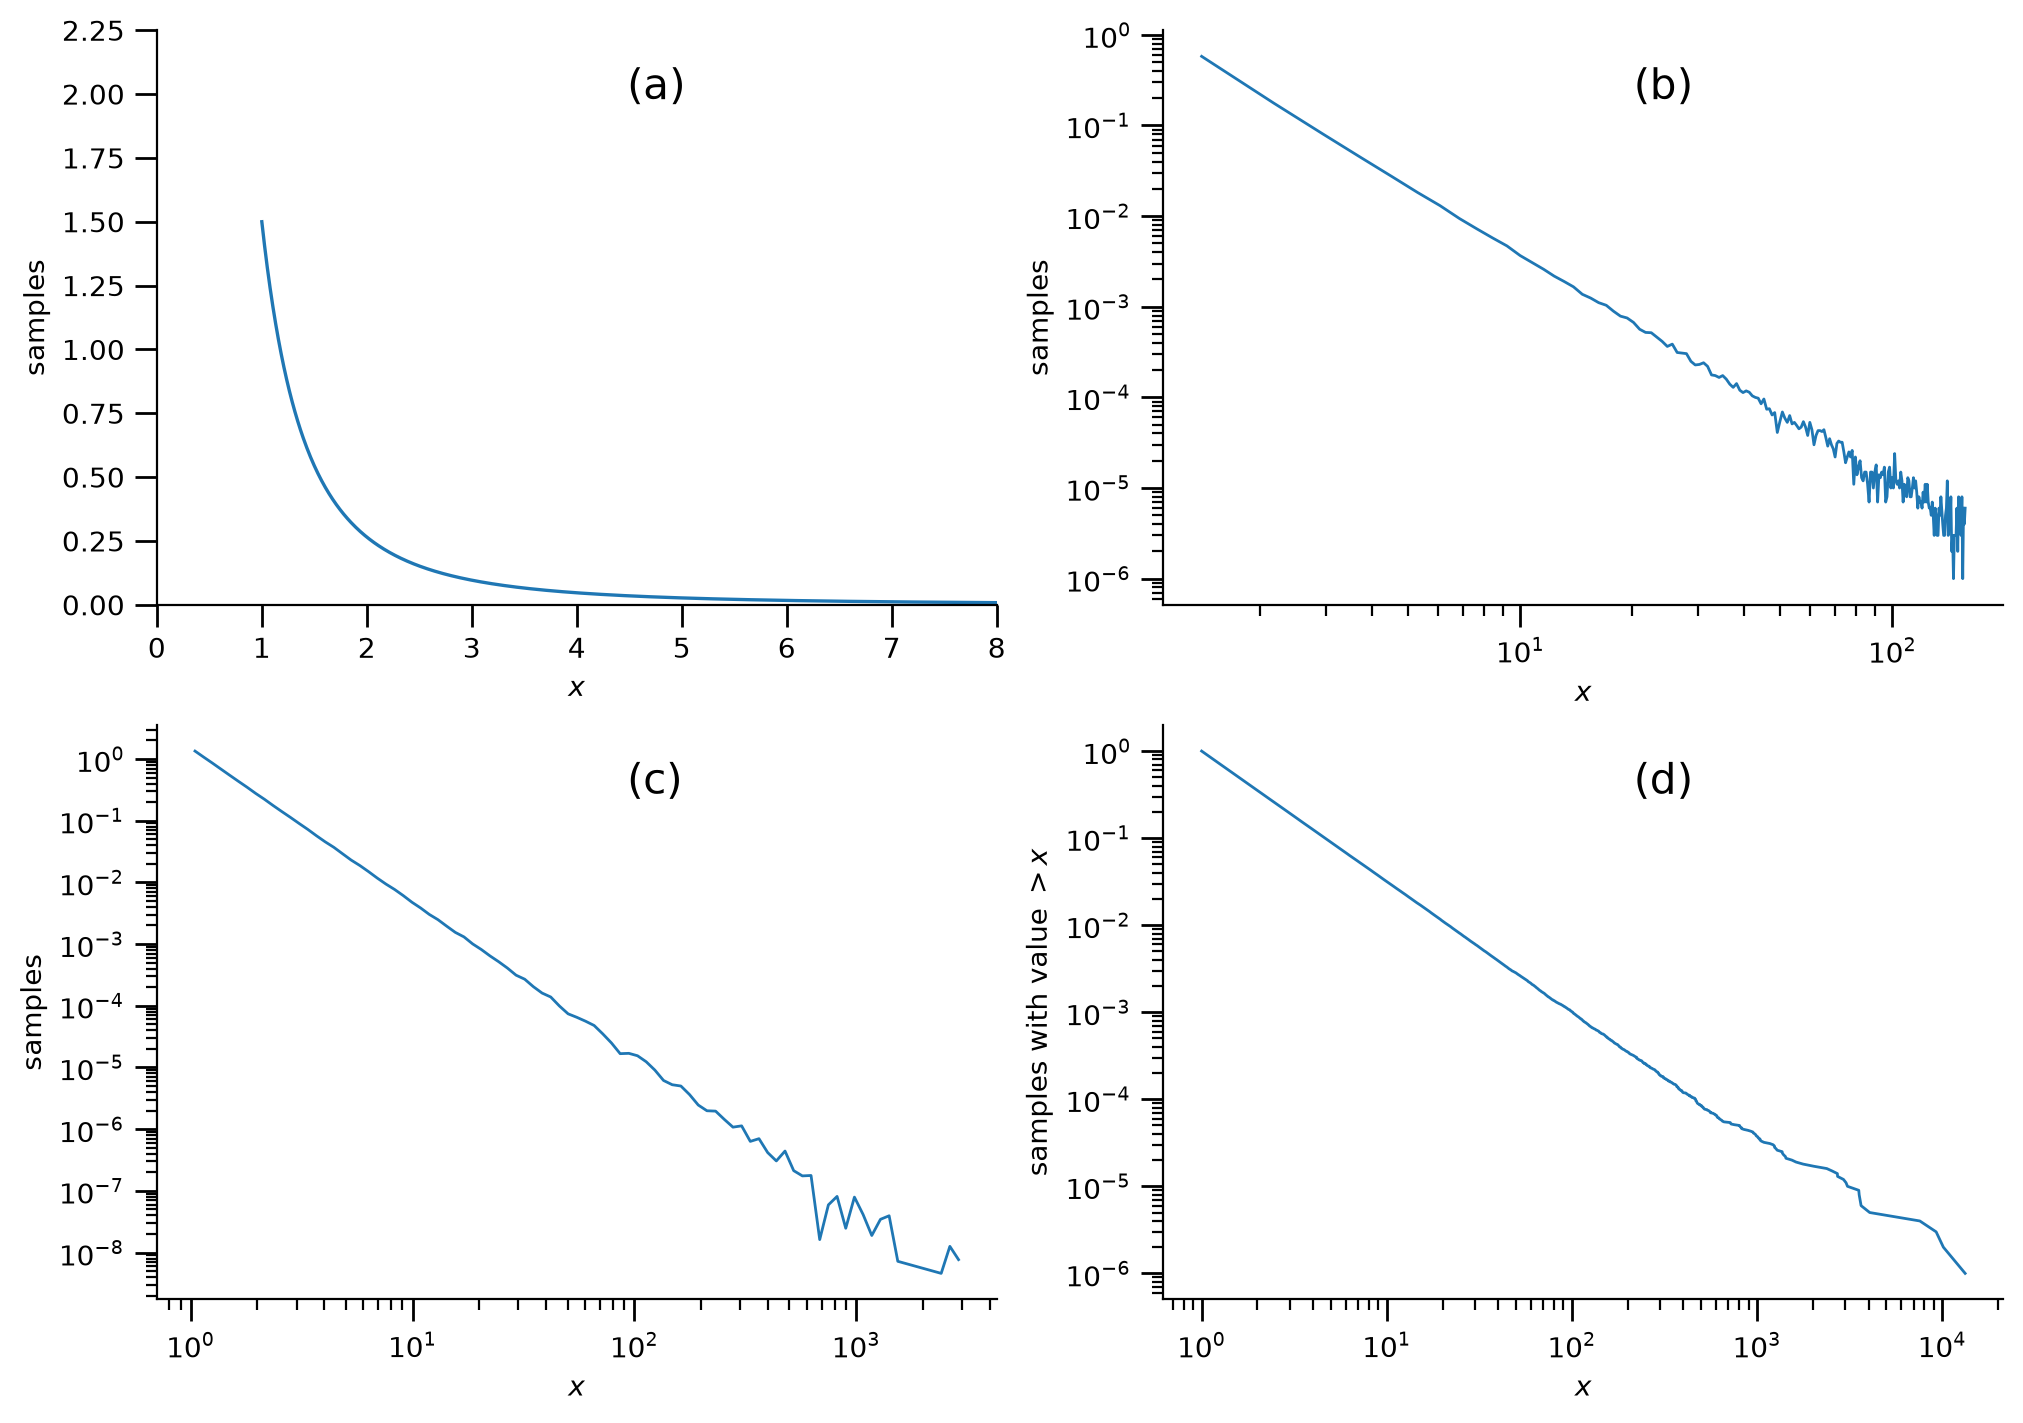
\includegraphics[width=0.72\textwidth]{newman_powerlaw_grid.png}
\caption{Four complementary representations of a synthetic power-law sample, following the pedagogical construction of Newman \cite{Newman2005}: linear representation, log--log representation with fixed linear-width aggregation, logarithmic-bin density, and empirical CCDF.}
\label{fig:newman-grid}
\end{figure}



\section{Numerical comparison of the binning methods}

This section applies the preceding definitions to controlled synthetic samples. All samples contain $N=10^6$ observations and all random draws use a fixed seed so that the numerical comparison is reproducible. We compare the occupancy structure produced by \texttt{cut}, \texttt{qcut}, and logarithmic binning, then examine the empirical CCDFs and the conditional mean within each bin. The results show that no method dominates for every purpose: quantile bins control occupancy, equal-width bins preserve additive resolution, and logarithmic bins preserve multiplicative resolution while substantially improving representation of broad tails.

\subsection{Binning results for the three methods}

Table~\ref{tab:binning-results} reports a compact numerical diagnostic for $K=50$ bins. The minimum and maximum occupancies and the number of empty bins measure how unevenly each partition distributes observations. To summarize this unevenness with a dimensionless quantity, we use the coefficient of variation (CV) of the bin occupancies,
\begin{equation}
 \mathrm{CV}=\frac{s_n}{\bar n},
 \qquad
 \bar n=\frac{1}{K}\sum_{k=1}^{K}n_k=\frac{n}{K},
\end{equation}
where $s_n$ is the standard deviation of the $K$ bin counts and $\bar n$ is their mean. Thus $\mathrm{CV}=0$ corresponds to exactly equal occupancies, while larger values indicate increasingly concentrated bin counts.

\begin{table}[htbp]
\centering
\caption{Occupancy diagnostics for $N=10^6$ observations and $K=50$ bins. CV denotes the coefficient of variation of the bin counts.}
\label{tab:binning-results}
\renewcommand{\arraystretch}{1.22}
\begin{tabular*}{0.98\textwidth}{@{\extracolsep{\fill}}llcccc@{}}
\toprule
Distribution & Method & Min. count & Max. count & Empty bins & CV \\
\midrule
Exponential & cut & $0$ & $245{,}434$ & $5$ & $2.451$ \\
Exponential & qcut & $20{,}000$ & $20{,}000$ & $0$ & $0.000$ \\
Exponential & log binning & $0$ & $119{,}337$ & $1$ & $1.761$ \\
Lognormal & cut & $0$ & $214{,}121$ & $2$ & $2.458$ \\
Lognormal & qcut & $20{,}000$ & $20{,}000$ & $0$ & $0.000$ \\
Lognormal & log binning & $1$ & $76{,}481$ & $0$ & $1.304$ \\
Pareto & cut & $0$ & $999{,}874$ & $40$ & $6.999$ \\
Pareto & qcut & $20{,}000$ & $20{,}000$ & $0$ & $0.000$ \\
Pareto & log binning & $0$ & $258{,}976$ & $6$ & $2.538$ \\
\bottomrule
\end{tabular*}
\end{table}

The quantile result is exact here because $10^6$ is divisible by $50$ and the simulated samples are continuous, so ties at the quantile edges occur with probability zero. Every \texttt{qcut} bin contains $20{,}000$ observations. This property is useful when subsequent statistics should be estimated from groups with comparable sample sizes, although the corresponding widths can differ enormously.

The equal-width result exposes the heavy-tail problem. For the Pareto sample, $999{,}874$ of the $10^6$ observations fall into the most populated equal-width bin and $40$ of the $50$ bins are empty. The maximum observation determines such a large range that a linear partition becomes almost useless for resolving the body of the sample. In this particular run, the documented $0.1\%$ range extension used by \texttt{pandas.cut} when \texttt{bins} is an integer even moves the numerical lower edge below zero, despite every Pareto observation being positive; this is an edge-construction artifact caused by the enormous full range, not a property of the data. Logarithmic binning is far less concentrated because the widths expand geometrically, although its purpose is not to equalize counts and some far-tail bins remain empty in a finite sample. For the lognormal sample, logarithmic binning is particularly effective at avoiding empty intervals while retaining multiplicative resolution.

The ordinary histograms in Fig.~\ref{fig:synthetic-histograms} provide the complementary visual picture. As $K$ increases, the exponential and lognormal distributions acquire progressively finer resolution, whereas the Pareto distribution continues to require a representation adapted to its long tail.

\subsection{Complementary cumulative distributions}

Figure~\ref{fig:ccdf-grid} compares the empirical CCDF with an illustrative log--log ordinary least-squares fit for each of the three synthetic distributions. The three rows repeat the same CCDF for $K=25$, $50$, and $100$ only to preserve visual correspondence with the binning experiments; the CCDF itself is independent of $K$. This independence is one of its principal advantages, because the cumulative representation is constructed directly from the ordered sample rather than from histogram boundaries.

\begin{figure}[!htbp]
\centering
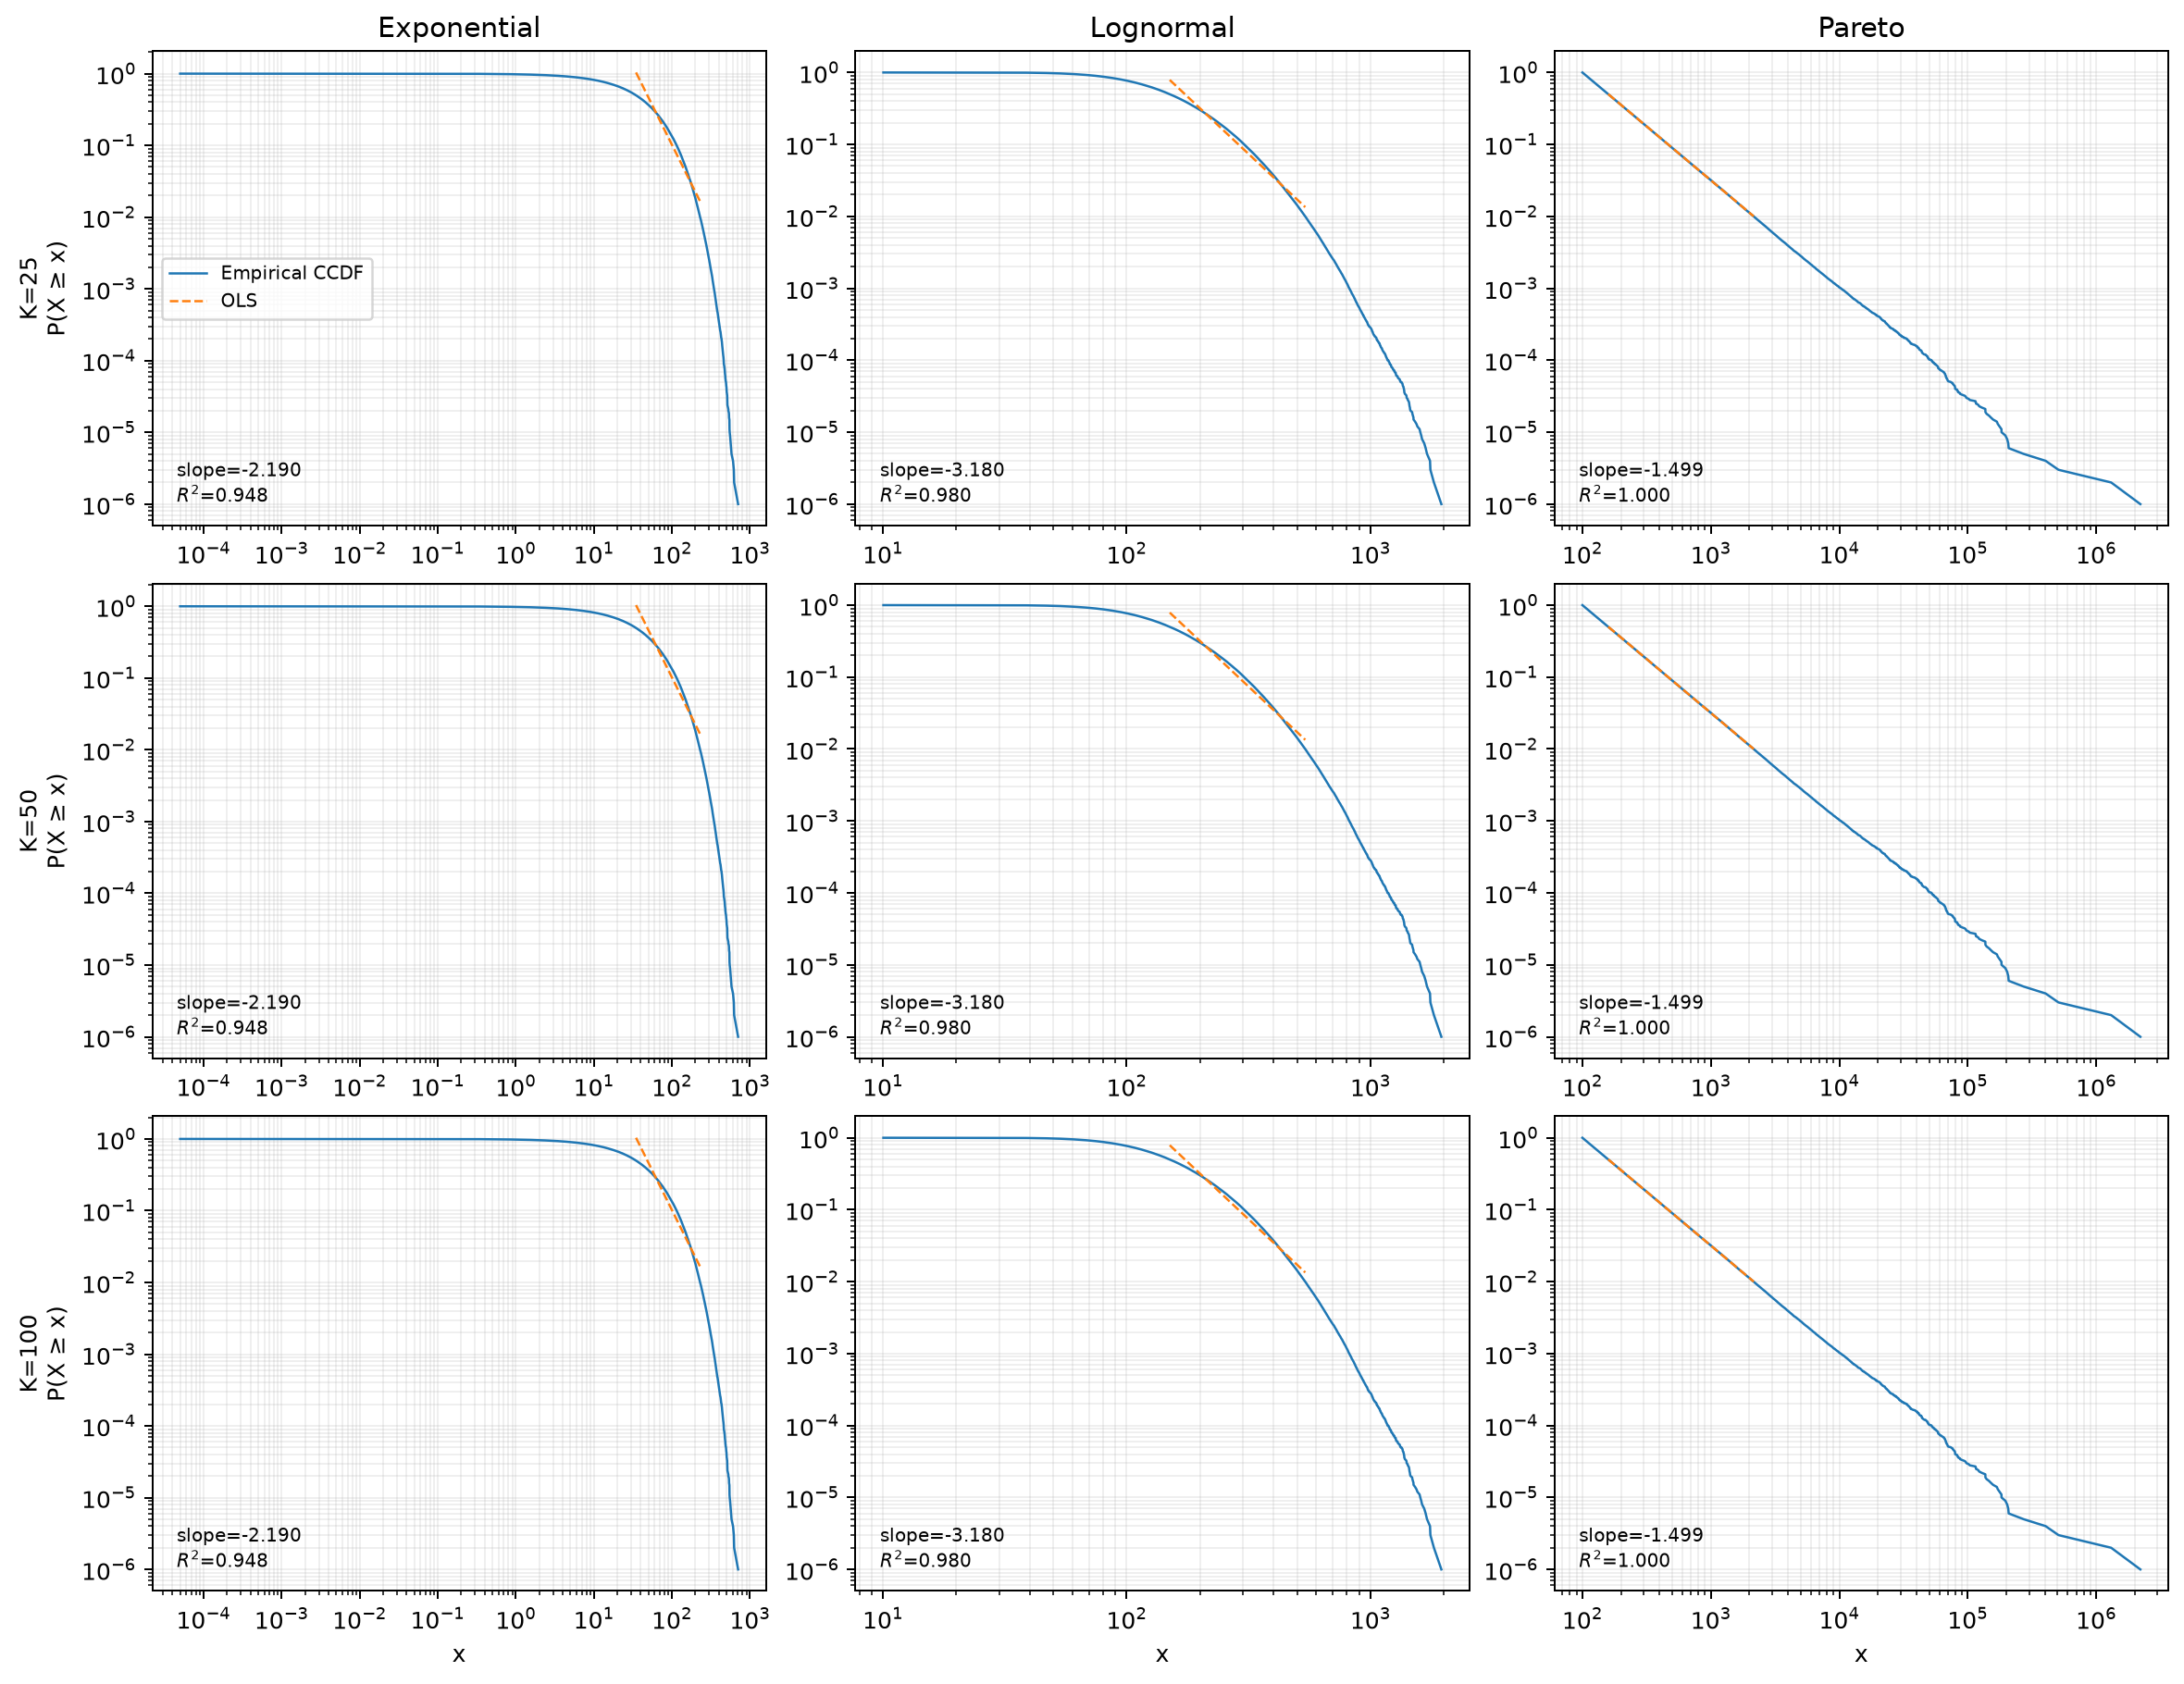
\includegraphics[width=0.92\textwidth]{assets/ccdf_grid_no_title.png}
\caption{Empirical complementary cumulative distributions for the exponential, lognormal, and Pareto samples. The repeated rows emphasize that the empirical CCDF is independent of the number of histogram bins. Dashed lines show an illustrative ordinary least-squares fit over a restricted survival-probability interval and should not be interpreted as a formal power-law test.}
\label{fig:ccdf-grid}
\end{figure}

For the exponential law,
\begin{equation}
 \overline F(x)=e^{-\lambda x},
\end{equation}
so a log--log plot is curved rather than linear. The lognormal CCDF is broad and may resemble a line over a limited interval, but it also develops systematic curvature. For the Pareto law in Eq.~\eqref{eq:pareto-ccdf},
\begin{equation}
 \log \overline F(x)
 =-(\alpha-1)\log x +(\alpha-1)\log x_{\min},
\end{equation}
which is exactly linear in log--log coordinates. With $\alpha=2.5$, the theoretical CCDF slope is $-1.5$.

The dashed ordinary least-squares lines in Fig.~\ref{fig:ccdf-grid} are included only as visual diagnostics. Clauset, Shalizi, and Newman \cite{ClausetShaliziNewman2009} show why least-squares regression on logarithmically transformed histograms or cumulative plots is generally inadequate for estimating and validating a power law. A proper empirical analysis should estimate the lower cutoff, fit the exponent by maximum likelihood, evaluate goodness of fit, and compare plausible alternative distributions.

\subsection{Mean value within each bin}

The mean of the observations assigned to a bin is a useful way to visualize what the partition does to the scale of the data. For bin $B_k$ with occupancy $n_k>0$, define
\begin{equation}
 \overline x_k
 =\frac{1}{n_k}\sum_{i:x_i\in B_k}x_i.
\end{equation}
Figure~\ref{fig:bin-means} plots this quantity against the bin index for the three methods, three distributions, and three values of $K$. The figure is the same reproducible asset generated by the numerical experiment pipeline; every panel contains its own legend so that the three binning methods remain identifiable without relying on another panel.

\begin{figure}[!htbp]
\centering
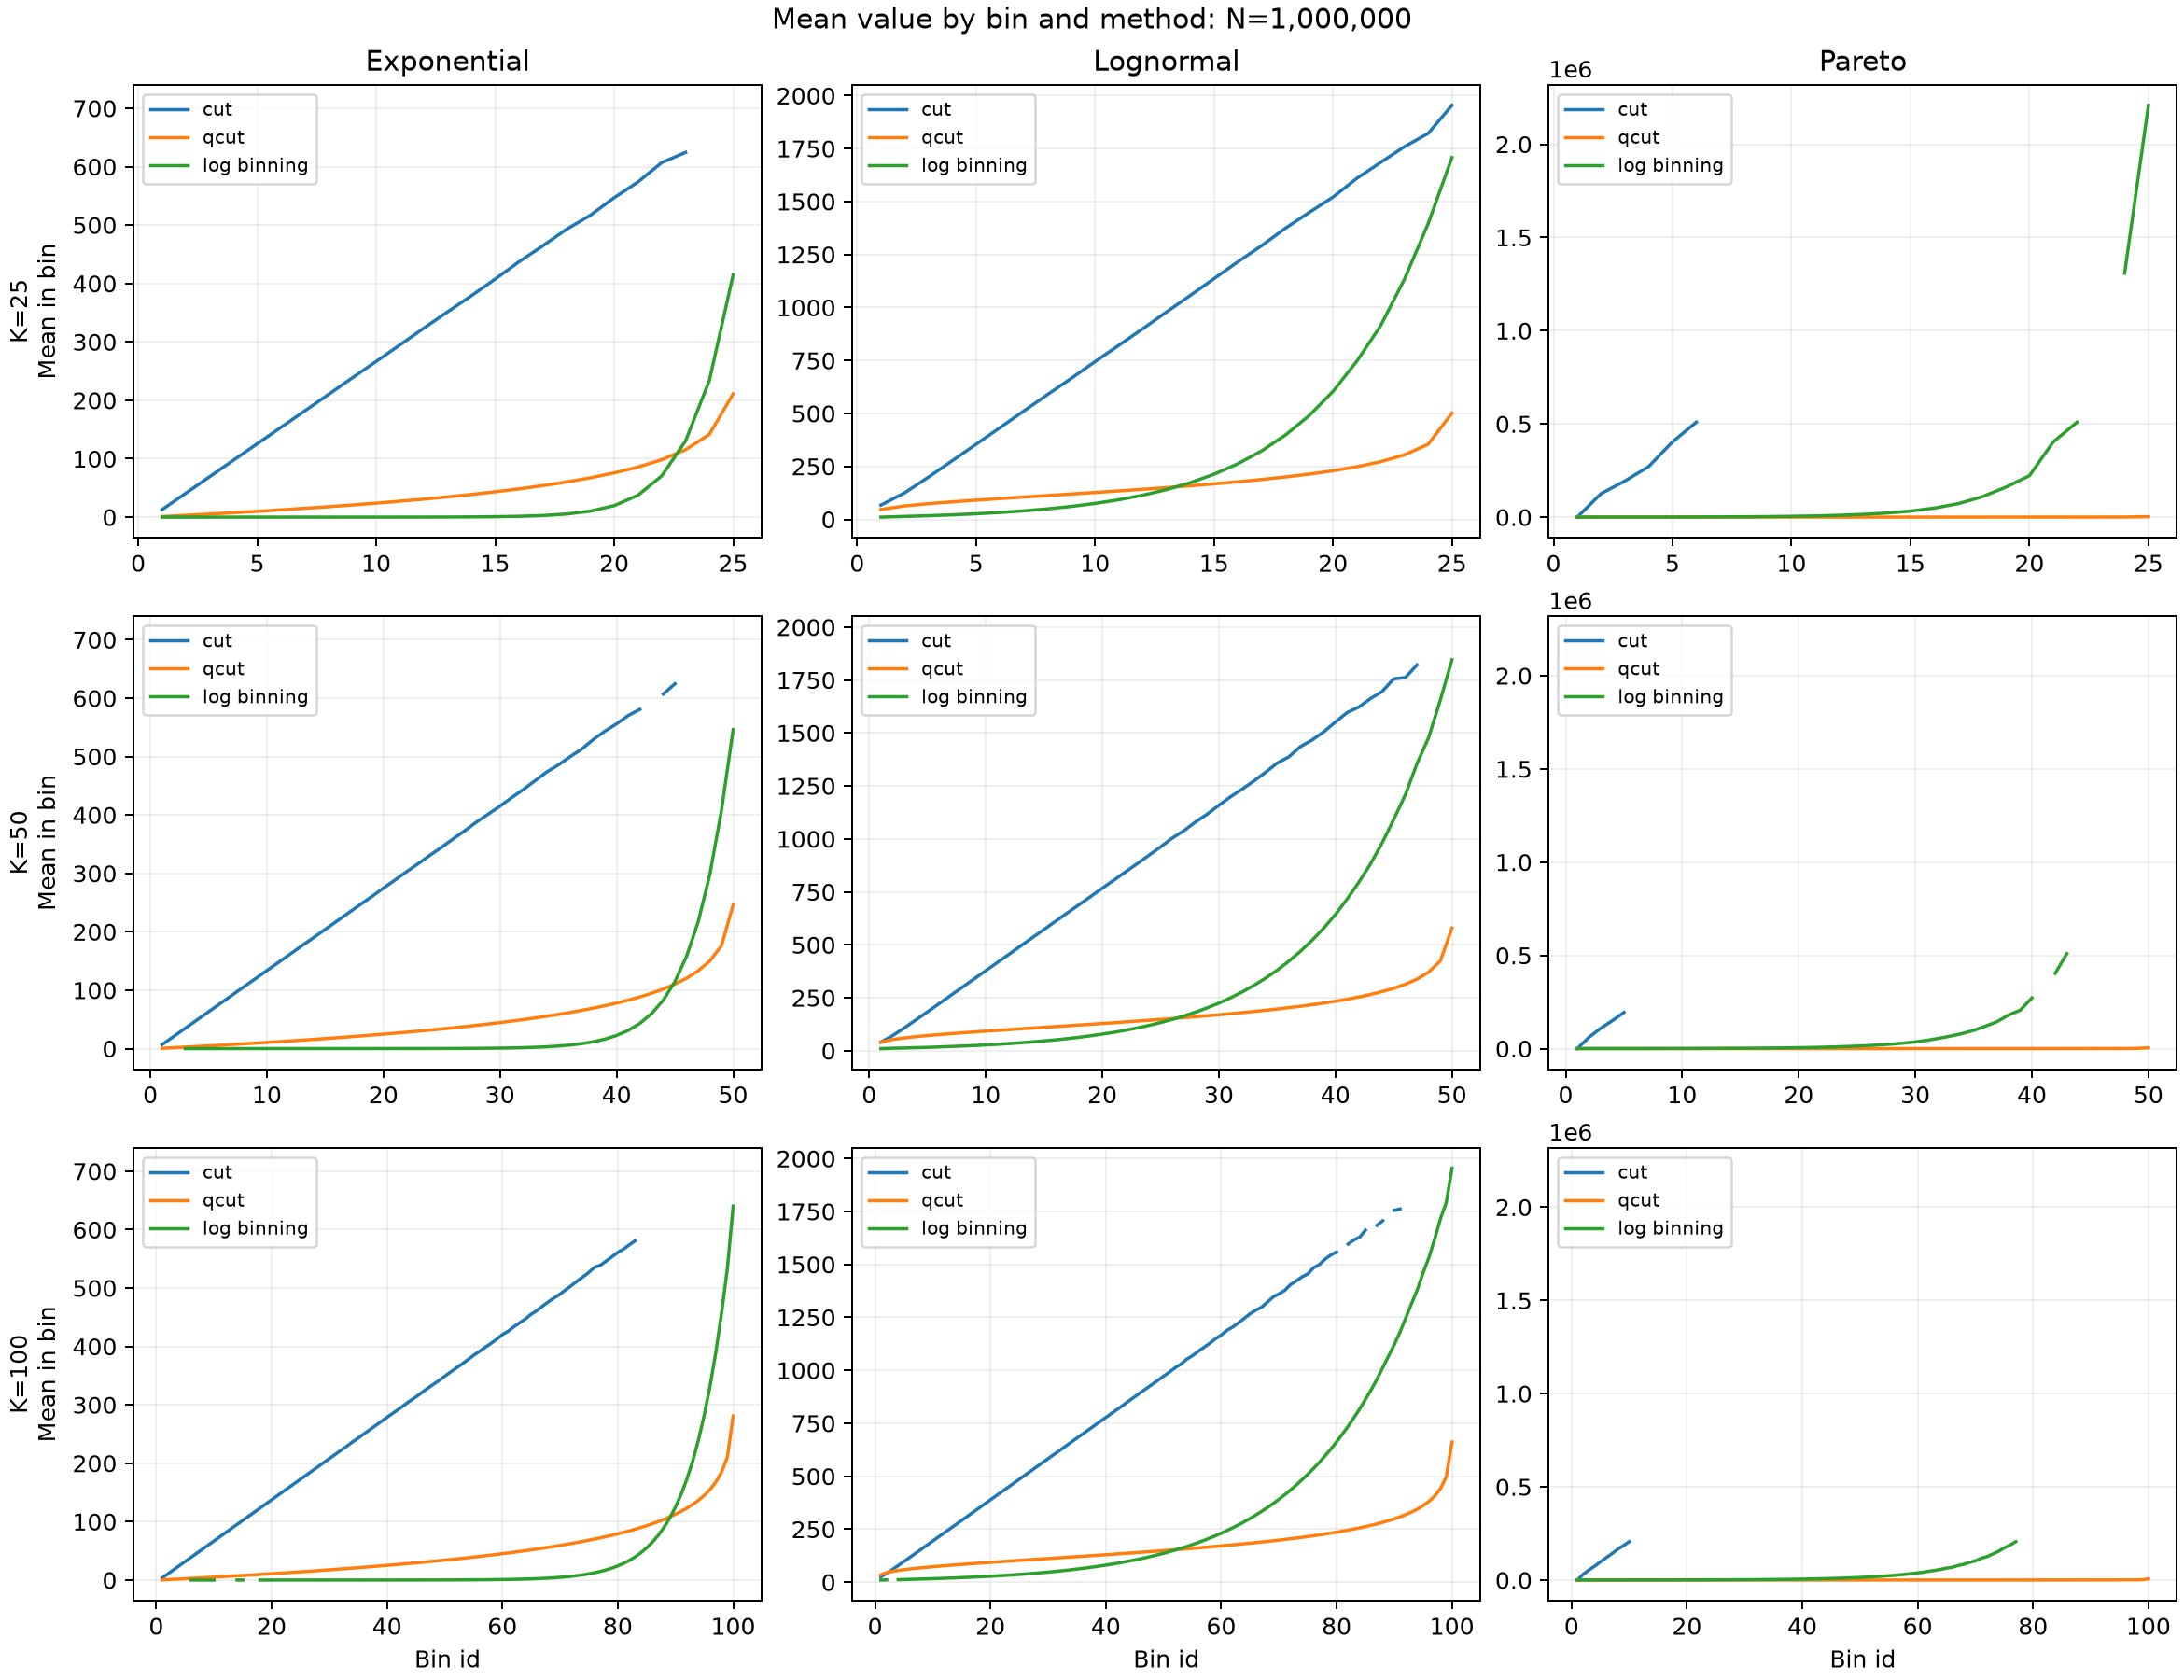
\includegraphics[width=0.92\textwidth]{bin_means_grid.png}
\caption{Mean observation within each bin for \texttt{cut}, \texttt{qcut}, and logarithmic binning. All nine panels use a linear vertical scale and contain their own legend.}
\label{fig:bin-means}
\end{figure}

The three curves have different interpretations because the index $k$ labels different geometries. Under \texttt{cut}, consecutive indices represent equal additive increments in $x$, so the mean of an occupied bin tends to track its interval center. Under \texttt{qcut}, consecutive indices represent equal increments of empirical probability, not equal increments of $x$. The upper quantile bins therefore become progressively wider for skewed data, and the final bin can have a mean much larger than the preceding bins. Under logarithmic binning, consecutive indices represent equal increments in $\log x$, so the characteristic scale of the bins grows geometrically.

The Pareto panels make the contrast most visible. The equal-width method produces a long sequence of sparse or empty high-index bins because a few extreme observations determine the total linear range. Quantile binning avoids empty groups by construction but places an increasingly broad interval into the upper quantiles. Logarithmic binning follows the multiplicative geometry of the tail and therefore distributes resolution more evenly across orders of magnitude. On a linear vertical axis, the extreme-bin means naturally dominate the Pareto panels; this is a genuine consequence of the long tail rather than a plotting defect.

Taken together, the results suggest a practical division of labor. Equal-width bins are appropriate when additive distances are the quantity of interest and the observed range is not dominated by extremes. Quantile bins are appropriate when comparable group sizes are required. Logarithmic bins are appropriate when positive data span several orders of magnitude and multiplicative resolution is more meaningful than additive resolution. The CCDF should be considered alongside all three because it retains the full ordering information without requiring any bin boundaries.


\section*{Code Availability}

All numerical experiments, synthetic-data generation routines, figure-generation functions, and the complete source of these lecture notes are publicly available at \url{https://github.com/ozsp12/notes_econophys} in the \texttt{log\_binning} directory. The repository contains the Python routines used to reproduce the histogram, CCDF, bin-mean, and Newman-style power-law figures, together with the numerical output table, the LaTeX source, and the BibTeX database. Manuscript-specific graphical assets are stored under \texttt{log\_binning/assets}; the Newman-style grid is additionally decomposed into four separately generated panel images so that its layout can be reproduced or rearranged without altering the underlying sample. Random-number generation uses fixed seeds so that the computational results reported here can be reproduced from the documented dependencies.


\bibliography{log_binning}
\bibliographystyle{unsrt}

\end{document}
